\documentclass[dvipdfmx]{jsarticle}

\title{西暦和暦変換プログラムの作成(Java版)}
\author{Seiichi Nukayama}
\date{2020-05-05}
\usepackage{tcolorbox}
\usepackage{color}
\usepackage{listings, plistings}

% Java
\lstset{% 
  frame=single,
  backgroundcolor={\color[gray]{.9}},
  stringstyle={\ttfamily \color[rgb]{0,0,1}},
  commentstyle={\itshape \color[cmyk]{1,0,1,0}},
  identifierstyle={\ttfamily}, 
  keywordstyle={\ttfamily \color[cmyk]{0,1,0,0}},
  basicstyle={\ttfamily},
  breaklines=true,
  xleftmargin=0zw,
  xrightmargin=0zw,
  framerule=.2pt,
  columns=[l]{fullflexible},
  numbers=left,
  stepnumber=1,
  numberstyle={\scriptsize},
  numbersep=1em,
  language={Java},
  lineskip=-0.5zw,
  morecomment={[s][{\color[cmyk]{1,0,0,0}}]{/**}{*/}},
}
%\usepackage[dvipdfmx]{graphicx}
\usepackage{url}
\usepackage[dvipdfmx]{hyperref}
\usepackage{amsmath, amssymb}
\usepackage{itembkbx}
\usepackage{eclbkbox}	% required for `\breakbox' (yatex added)
\fboxrule=1pt
\parindent=1em
\begin{document}

\pagenumbering{arabic}

%% 修正時刻: Wed May  6 07:18:47 2020


\section{解答例}

\subsection{Eclipseを使わないやり方}

\subsubsection{ディレクトリの作成場所とTomcatへの登録}

ディレクトリを以下のようにする。

\begin{tcolorbox}
 /home/\$HOME/work/Lala/jsp/nengo
\end{tcolorbox}

これをTomcatに登録する。

\verb!$CATALINA_HOME/conf/Catalina/localhost! に以下のファイルをおく。

\begin{lstlisting}[caption=nengo.xml]
 <?xml version="1.0" encoding="utf-8" ?>
 <Context path="/nengo" docBase="/home/(ユーザー名)/work/Lala/jsp/nengo" />
\end{lstlisting}

\verb!/home/$HOME/work/Lala/jsp/nengo! を以下のように構成する。

\begin{verbatim}
./
├── WEB-INF
│   ├── classes
│   ├── lib
│   └── web.xml
├── css
│   └── nengo.css
├── index.jsp
└── src
     └── com
         └── example
             └── nengo
                 ├── Nengo.java
                 └── Xnengo.java
\end{verbatim}

\subsubsection{初期ファイル}

web.xml は以下のようにする。

\begin{lstlisting} [caption=web.xml]
 <?xml version="1.0" encoding="UTF-8" ?>
<web-app>
    <servlet>
        <servlet-name>nengo</servlet-name>
        <servlet-class>com.example.nengo.Nengo</servlet-class>
    </servlet>
    <servlet-mapping>
        <servlet-name>nengo</servlet-name>
        <url-pattern>/nengo</url-pattern>
    </servlet-mapping>
</web-app>
\end{lstlisting}

index.jsp は以下のようにする。

\begin{lstlisting} [caption=index.jsp]
<%@ page language="java" contentType="text/html; charset=UTF-8"
         pageEncoding="UTF-8" %>
<!doctype html>
<html lang="ja">
  <head>
    <meta charset="utf-8"/>
    <title>年号変換プログラム</title>
    <link rel="stylesheet" href="css/nengo.css"/>
  </head>
  <body>
    <div id="wrap">
      <header>
        <h1>年号変換プログラム</h1>
      </header>
      <article>
        <section>
          <h1>西暦⇒年号</h1>
          <form action="/nengo/Xnengo" method="post">
            <p>西暦年を入力してください</p>
            <p><input type="text" name="seireki" id="seireki"/>年
              &nbsp;&nbsp;
              <input type="submit" value="年号を調べる"/></p>
          </form>
          <div id="kaito-nengo"></div>
        </section>
        <section>
          <h1>年号→西暦</h1>
          <form action="/nengo/Xnengo" method="post">
            <p>年号と年を入力してください</p>
            <p><select name="nengo" id="nengo">
              <option value="" selected>選択してください</option>
              <option value="meiji">明治</option>
              <option value="taisyo">大正</option>
              <option value="syouwa">昭和</option>
              <option value="heisei">平成</option>
              <option value="reiwa">令和</option>
              <option value="mirai">未来</option>
            </select>
            &nbsp;&nbsp;
            <input type="text" name="nen" id="nen"/>年
            &nbsp;&nbsp;
            <input type="submit" value="西暦を調べる"/></p>
          </form>
          <div id="kaito-seireki"></div>
        </section>
      </article>
      <footer>
        <small>Copyright &copy; 2020 Seiichi Nukayama</small>
      </footer>
    </div>
  </body>
</html>
\end{lstlisting}

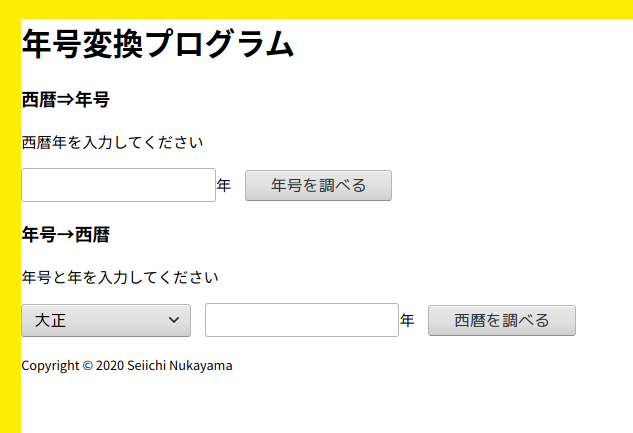
\includegraphics[width=10cm]{gamen01.png}

さて、index.jsp からポストされたデータは、com.example.nengo.Xnengo サー
ブレットで受け取る。

 \begin{lstlisting} [caption=WEB-INF/src/com/example/nengo/Xnengo.java]
// Xnengo.java
package com.example.nengo;

import javax.servlet.*;
import javax.servlet.http.*;
import java.io.*;
import java.util.*;

public class Xnengo extends HttpServlet {
    private static final long serialVersionUID = 1L;

    private int seireki = 0;
    private String nengo = "";
    private int nen = 0;
    private final String ERROR = "エラーです";
    
    
    protected void doPost( HttpServletRequest request, HttpServletResponse response )
        throws ServletException, IOException {
        request.setCharacterEncoding("UTF-8");

        HttpSession session = request.getSession(true);
        
        String txtSeireki = request.getParameter("seireki");
        if (txtSeireki != null && txtSeireki != "") {
            this.toNengo(txtSeireki);
            session.setAttribute("nengo", this.nengo);
            session.setAttribute("nen", this.nen);
            session.setAttribute("error", null);
        } else {
            session.setAttribute("nengo", null);
            session.setAttribute("nen", null);
            session.setAttribute("error", this.ERROR);
        }
        response.sendRedirect("/nengo");
    }

    private void toNengo(String txtSeireki) {
        int s = Integer.parseInt(txtSeireki);
        Nengo n = new Nengo();
        n.toNengo(s);
        this.nengo = n.getNengo();
        this.nen = n.getNen();
    }
} 
 \end{lstlisting}




\end{document}

%% 修正時刻: Sat May  2 15:10:04 2020


%% 修正時刻: Tue May 12 06:50:51 2020
